\documentclass{article}
\usepackage[a4paper, margin=2.5cm]{geometry}
\usepackage{polski, graphicx, float, hyperref}
\setcounter{secnumdepth}{0}

\begin{document}
\subsection{Podział architektury systemu}
System integracji drona neopixel sharky jest podzielony na 2 główne części:
\begin{itemize}
    \item Dodanie aparatury 5G na pokładzie drona
    \item Stworzenie stacji naziemnej do obsługi drona
\end{itemize}

\subsection{Aparatura 5G na pokładzie drona}
\subsubsection{Wykorzystany sprzęt}

\begin{itemize}
    \item Bramka 5G - RM500x / RM502x 5G HAT
    \item Raspberry Pi 4
    \item Kamera ip - ms-c9674-pa
\end{itemize}

\subsubsection{Schemat blokowy}
Kolorem niebieskim zaznaczono elementy, które są dokładne do drona w ramach projektu\\
Kolorem zielonynm zaznaczono elementy, które są już obecne.

\begin{figure}[H]
    \centering
    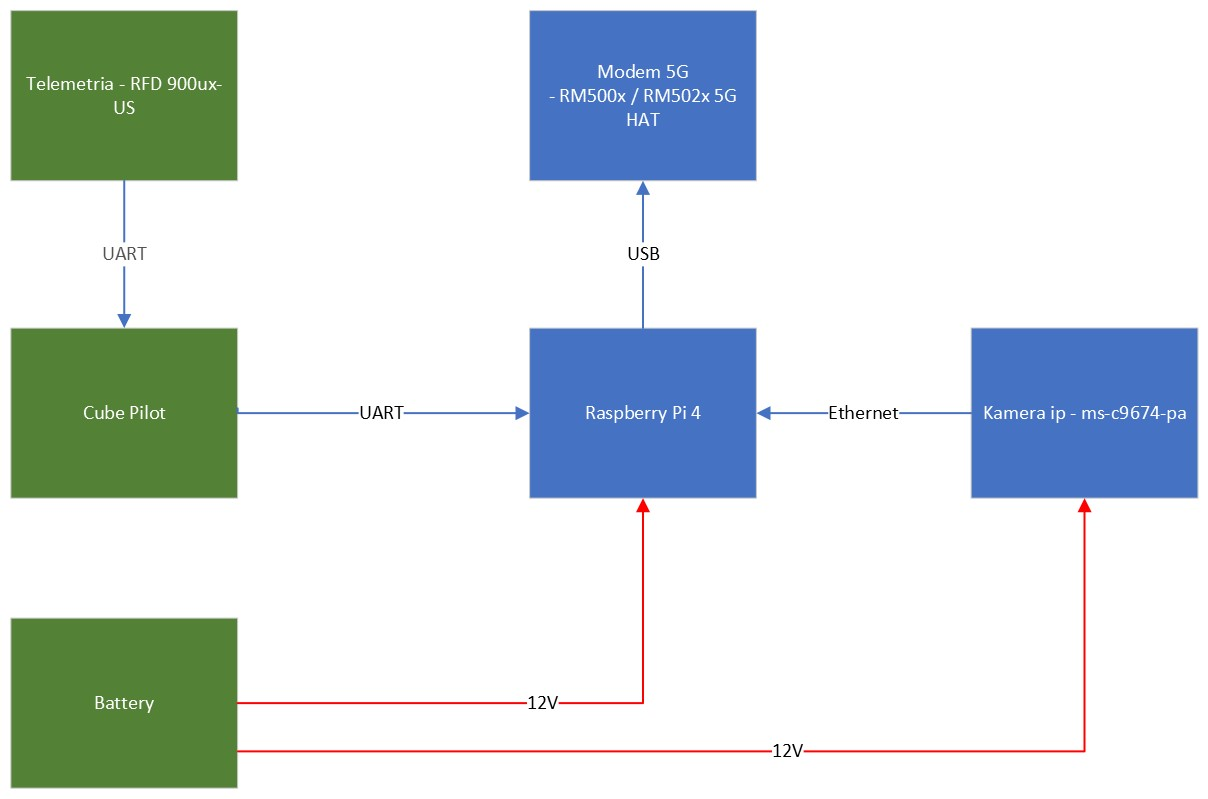
\includegraphics[width=0.9\textwidth]{nadronie.jpg}
    \caption{Schemat blokowy części na dronie}
\end{figure}

\subsubsection{Opis działania}
Na dronie obecnie się znajduje moduł cube pilot na którym działa oprogramowanie ardupilot. W celu integracji z modułem 5G, należy podłączyć go do raspberry pi 4.
Cube pilot i raspberry pi 4 komunikują się ze sobą za pomocą portu szergowego. Raspberry pi 4 jest podłączone do kamery ip za pomocą portu ethernet. Do modemu 5G raspberry pi jest podłączone kablem usb. 
Zadaniem raspberry pi jest zamiana danych z kamery ip na format, który może być przesyłany przez modem 5G. Zamienia również dane przesyłane MAVlinkiem z cube pilota na UDP, za pomocą oprogramowania mavproxy.
Wszystkie moduły są zasilane z baterii drona.

\subsubsection{Problemy do rozwiązania}
Trzeba znaleść lub napisać oprogramowanie zdolne przetworzyć dane z kamery ip na format, który może być przesyłany przez modem 5G w czasie rzeczywistym.
Sparawdzić czy układy nie wymagają dołożenia odzielnego zasilacza z wyższą wydajnością prądową.

\subsection{Stacja naziemna}
\subsubsection{Wykorzystany sprzęt}
\begin{itemize}
    \item Bramka 5G
    \item komputer przemysłowy
    \item 2 x joystick
    \item Monitor
    \item Przyciski do sterowania
    \item Włącznik zasilania
    \item Przełącznik uzbrojenia
\end{itemize}

\subsubsection{Schemat blokowy}


\begin{figure}[H]
    \centering
    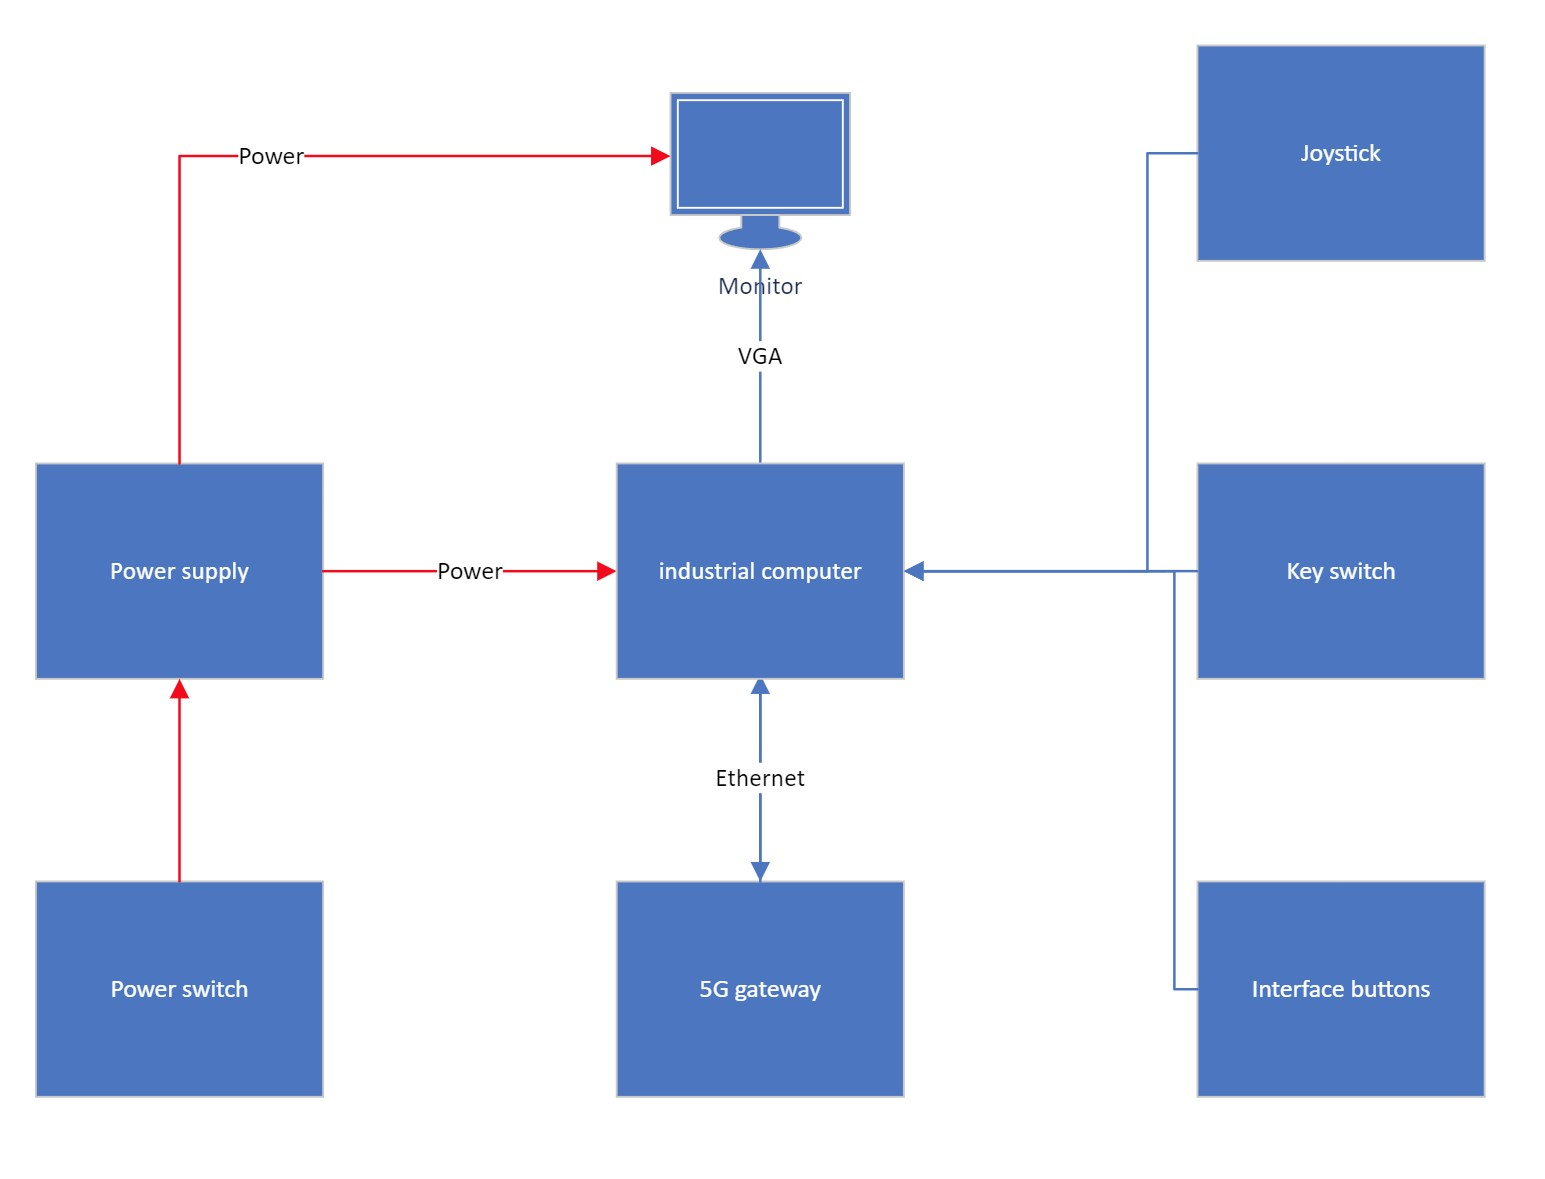
\includegraphics[width=0.9\textwidth]{stacja.jpg}
    \caption{Schemat blokowy części w stacji naziemnej}
\end{figure}

\subsubsection{Opis działania}
Stacja ma zadanie służyć za interfejs użytkownika do sterowania dronem.
Ma za zadanie odbierać dane z drona i wyświetlać je na monitorze oraz przekazywać dane z joysticków do drona.
Ma być również wyposażona w przycisk uzbrojenia, który będzie wysyłał sygnał do drona, żeby uzbroić drona oraz przycisk do awaryjnego wyłączenia drona.
Sercem stacji będzie komputer przemysłowy, który będzie odbierał dane z modemu 5G i przekazywał je do programu QGroundControl, który będzie wyświetlał dane na monitorze.
Możliwe jest również zastosowanie dodatkowe mikrokontrolera do komunikacji z peryferiami, takimi jak joysticki, przyciski, przełączniki, któty będzie się komunikował z komputerem przemysłowym za pomocą portu szeregowego.

\subsubsection{Problemy do rozwiązania}
Na obecnym etapie trzeba dobrać konkretne komopotenty, które będą spełniały wymagania projektu.

\end{document}
